\documentclass[aspectratio=169]{beamer}
\usetheme{Madrid}
\usecolortheme{default}
\usepackage[utf8]{inputenc}
\usepackage[T5]{fontenc}
\usepackage{graphicx}
\usepackage{hyperref}
\usepackage{booktabs}
\usepackage{amsmath}
\usepackage{listings}
\usepackage{xcolor}

\definecolor{codegreen}{rgb}{0,0.6,0}
\definecolor{codegray}{rgb}{0.5,0.5,0.5}
\definecolor{codepurple}{rgb}{0.58,0,0.82}
\definecolor{backcolour}{rgb}{0.95,0.95,0.92}

\lstdefinestyle{mystyle}{
    backgroundcolor=\color{backcolour},   
    commentstyle=\color{codegreen},
    keywordstyle=\color{magenta},
    numberstyle=\tiny\color{codegray},
    stringstyle=\color{codepurple},
    basicstyle=\ttfamily\footnotesize,
    breakatwhitespace=false,         
    breaklines=true,                 
    captionpos=b,                    
    keepspaces=true,                 
    numbers=left,                    
    numbersep=5pt,                  
    showspaces=false,                
    showstringspaces=false,
    showtabs=false,                  
    tabsize=2
}
\lstset{style=mystyle}

\setbeamertemplate{caption}[numbered]
\renewcommand{\figurename}{Hình}
\renewcommand{\thefigure}{2.\arabic{figure}}

\title[Chương 2: Toán học của NN]{Học Sâu (Deep Learning) \\ \vspace{0.5cm} \Large Chương 2: Các khối xây dựng toán học của Mạng Nơ-ron}
\author{Đại học Đông Á}
\date{\today}

\begin{document}

\begin{frame}
    \titlepage
\end{frame}

\begin{frame}{Nội dung chương}
    \tableofcontents
\end{frame}

% ---------------------------------------------
\section{1. Cái nhìn đầu tiên về mạng nơ-ron}
% ---------------------------------------------

\begin{frame}{Ví dụ kinh điển: Tập dữ liệu MNIST}
    \begin{columns}
        \column{0.5\textwidth}
        \begin{itemize}
            \item \textbf{Bài toán:} Phân loại ảnh các chữ số viết tay (từ 0 đến 9).
            \item \textbf{Dữ liệu:} $60.000$ ảnh huấn luyện, $10.000$ ảnh kiểm tra.
            \item Kích thước mỗi ảnh: $28 \times 28$ pixels (ảnh xám đen trắng).
            \item Trong học máy: 
            \begin{itemize}
                \item Phân loại (Category) gọi là \textbf{Lớp (Class)}.
                \item Dữ liệu đầu vào gọi là \textbf{Mẫu (Sample)}.
                \item Kết quả của mẫu gọi là \textbf{Nhãn (Label)}.
            \end{itemize}
        \end{itemize}
        
        \column{0.5\textwidth}
        \begin{figure}
            \centering
            
\includegraphics[width=\textwidth,height=0.7\textheight,keepaspectratio]{../../images/ch02/MNIST-sample-digits.3d651e1d.png}
            \caption{Một số mẫu ảnh từ MNIST}
        \end{figure}
    \end{columns}
\end{frame}

\begin{frame}[fragile]{Tải dữ liệu MNIST trong Keras}
    \begin{itemize}
        \item Tập dữ liệu MNIST được tải sẵn trong Keras, dưới dạng 4 mảng NumPy.
    \end{itemize}
    \begin{lstlisting}[language=Python]
from keras.datasets import mnist
(train_images, train_labels), (test_images, test_labels) = mnist.load_data()
    \end{lstlisting}
    \begin{itemize}
        \item \textbf{Tập huấn luyện (Training set):} \texttt{train\_images} và \texttt{train\_labels}
        \item \textbf{Tập kiểm tra (Test set):} \texttt{test\_images} và \texttt{test\_labels}
        \item Hình ảnh được mã hóa dưới dạng mảng NumPy, nhãn là các số từ $0$ đến $9$.
    \end{itemize}
\end{frame}

\begin{frame}[fragile]{Khám phá hình dạng dữ liệu}
    \begin{itemize}
        \item Mảng NumPy là thư viện phổ biến để tính toán số. Nó được sử dụng làm định dạng lưu trữ trao đổi dữ liệu.
        \item Hãy xem xét cấu trúc của tập huấn luyện:
    \end{itemize}
    \begin{lstlisting}[language=Python]
>>> train_images.shape
(60000, 28, 28)
>>> len(train_labels)
60000
>>> test_images.shape
(10000, 28, 28)
    \end{lstlisting}
    \begin{itemize}
        \item Dữ liệu huấn luyện gồm $60.000$ mẫu, mỗi mẫu là một ma trận $28 \times 28$.
    \end{itemize}
\end{frame}

\begin{frame}{Xem xét một mẫu dữ liệu (Sample)}
    \begin{columns}
        \column{0.5\textwidth}
        \begin{itemize}
            \item Mỗi bức ảnh là một ma trận số nguyên.
            \item Giá trị từ $0$ (trắng) đến $255$ (đen).
            \item Ở đây chúng ta hiển thị mẫu thứ 4 trong tập huấn luyện (chữ số '9').
        \end{itemize}
        
        \column{0.5\textwidth}
        \begin{figure}
            \centering
            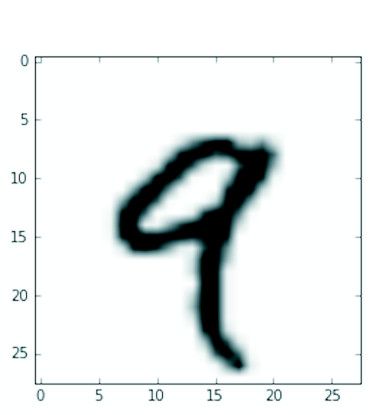
\includegraphics[width=\textwidth,height=0.7\textheight,keepaspectratio]{../../images/ch02/The-fourth-sample-in-our-dataset.8685ed9a.png}
            \caption{Biểu diễn ma trận của một ảnh}
        \end{figure}
    \end{columns}
\end{frame}

\begin{frame}[fragile]{Kiến trúc của mô hình mạng nơ-ron}
    \begin{itemize}
        \item Khối xây dựng cốt lõi của mạng nơ-ron là \textbf{lớp (layer)}. 
        \item Các lớp trích xuất các biểu diễn từ dữ liệu được cung cấp.
    \end{itemize}
    \begin{lstlisting}[language=Python]
import keras
from keras import layers

model = keras.Sequential(
    [
        layers.Dense(512, activation="relu"),
        layers.Dense(10, activation="softmax"),
    ]
)
    \end{lstlisting}
    \begin{itemize}
        \item Lớp \texttt{Dense} là lớp được kết nối đầy đủ (fully connected).
        \item Lớp cuối cùng là \texttt{softmax} 10 chiều, trả về mảng 10 điểm xác suất.
    \end{itemize}
\end{frame}

\begin{frame}[fragile]{Biên dịch (Compile) và Tiền xử lý dữ liệu}
    \begin{columns}
        \column{0.45\textwidth}
        \textbf{Biên dịch mô hình:}
        \begin{lstlisting}[language=Python]
model.compile(
    optimizer="adam",
    loss="sparse_categorical_crossentropy",
    metrics=["accuracy"],
)
        \end{lstlisting}
        
        \column{0.55\textwidth}
        \textbf{Tiền xử lý dữ liệu:} \\
        Biến đổi ảnh $28 \times 28$ thành vector $784$ chiều, đưa giá trị về khoảng $[0, 1]$.
        \begin{lstlisting}[language=Python]
train_images = train_images.reshape((60000, 28 * 28))
train_images = train_images.astype("float32") / 255
        \end{lstlisting}
    \end{columns}
\end{frame}

\begin{frame}[fragile]{Huấn luyện (Training) và Đánh giá (Evaluation)}
    \begin{itemize}
        \item Quá trình huấn luyện (khớp dữ liệu) trong Keras được thực hiện thông qua \texttt{model.fit()}.
    \end{itemize}
    \begin{lstlisting}[language=Python]
model.fit(train_images, train_labels, epochs=5, batch_size=128)
    \end{lstlisting}
    \begin{itemize}
        \item Sau khi huấn luyện, chúng ta đánh giá mô hình trên tập kiểm tra:
    \end{itemize}
    \begin{lstlisting}[language=Python]
test_loss, test_acc = model.evaluate(test_images, test_labels)
print(f"test_acc: {test_acc}") # Khoang 97.8%
    \end{lstlisting}
    \begin{itemize}
        \item Hiện tượng mô hình hoạt động kém hơn trên dữ liệu mới so với dữ liệu huấn luyện gọi là \textbf{Overfitting} (Quá khớp).
    \end{itemize}
\end{frame}

% ---------------------------------------------
\section{2. Biểu diễn dữ liệu bằng Tensor}
% ---------------------------------------------

\begin{frame}{Định nghĩa Tensor (Bộ căng)}
    Trong học sâu, mọi dữ liệu đều được biểu diễn thông qua các mảng đa chiều gọi là \textbf{Tensor}.
    \begin{itemize}
        \item \textbf{Vô hướng (Scalar) - Tensor 0D:} Chỉ chứa một con số duy nhất. Ví dụ: \texttt{np.array(12)}. Có 0 trục.
        \item \textbf{Vector - Tensor 1D:} Một mảng các con số. Trục duy nhất biểu diễn số chiều của vector.
        \item \textbf{Ma trận (Matrix) - Tensor 2D:} Một mảng của các vector (có Hàng và Cột).
        \item \textbf{Tensor 3D:} Đóng gói các ma trận thành hình hộp.
        \item \textbf{Tensor 4D, 5D:} Ứng dụng phổ biến cho chuỗi video.
    \end{itemize}
\end{frame}

\begin{frame}{Các thuộc tính chính của Tensor}
    Một tensor được xác định bởi ba thuộc tính cốt lõi:
    \begin{enumerate}
        \item \textbf{Số trục (thứ hạng - rank):} Được biểu thị bằng \texttt{ndim} trong NumPy. Một ma trận có 2 trục, Tensor 3D có 3 trục.
        \item \textbf{Hình dạng (shape):} Là một tuple chứa số nguyên mô tả số chiều dọc theo mỗi trục. Ví dụ: $(60000, 28, 28)$.
        \item \textbf{Kiểu dữ liệu (dtype):} Loại dữ liệu chứa trong tensor (\texttt{float32}, \texttt{uint8}, \texttt{float64}, \texttt{bool} v.v...).
    \end{enumerate}
\end{frame}

\begin{frame}[fragile]{Thao tác với Tensor: Cắt (Slicing) và Khái niệm Lô (Batch)}
    \begin{itemize}
        \item \textbf{Cắt Tensor (Slicing):} Lựa chọn phần tử cụ thể dọc theo các trục.
    \end{itemize}
    \begin{lstlisting}[language=Python]
my_slice = train_images[10:100] # Chon tu index 10 den 99
# Tuong duong: train_images[10:100, :, :]
# Cat o giua buc anh 14x14:
my_slice = train_images[:, 7:-7, 7:-7] 
    \end{lstlisting}
    \begin{itemize}
        \item \textbf{Khái niệm Lô (Batch):} Mô hình học sâu xử lý dữ liệu theo các đợt nhỏ. Trục đầu tiên (trục 0) thường được gọi là \textbf{trục lô (batch axis)}.
    \end{itemize}
    \begin{lstlisting}[language=Python]
batch = train_images[:128] # Lo dau tien gom 128 mau
    \end{lstlisting}
\end{frame}

\begin{frame}{Ví dụ thực tế: Vector và Dữ liệu Chuỗi thời gian}
    \begin{columns}
        \column{0.5\textwidth}
        \textbf{Dữ liệu Chuỗi thời gian (Tensor 3D)}
        \begin{itemize}
            \item Hình dạng: \texttt{(mẫu, thời gian, đặc trưng)}
            \item Trục thời gian luôn là trục thứ hai (index 1).
            \item \textit{Ví dụ:} Giá cổ phiếu mỗi phút (hiện tại, cao nhất, thấp nhất) trong 390 phút, 250 ngày giao dịch $\rightarrow$ Tensor \texttt{(250, 390, 3)}.
        \end{itemize}
        
        \column{0.5\textwidth}
        \begin{figure}
            \centering
            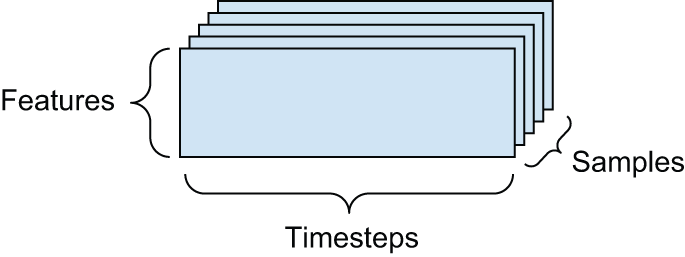
\includegraphics[width=\textwidth,height=0.7\textheight,keepaspectratio]{../../images/ch02/timeseries_data.a711cc5a.png}
            \caption{Tensor 3D cho dữ liệu chuỗi thời gian}
        \end{figure}
    \end{columns}
\end{frame}

\begin{frame}{Ví dụ thực tế: Dữ liệu Ảnh}
    \begin{columns}
        \column{0.5\textwidth}
        Ảnh kỹ thuật số thường có 3 chiều: Chiều cao, Chiều rộng và Kênh màu.
        \begin{itemize}
            \item \textbf{Lô ảnh (Batch of images):} Tạo thành một \textbf{Tensor 4D}.
            \item Hình dạng: \texttt{(mẫu, chiều cao, chiều rộng, kênh màu)}
            \item \textit{Ví dụ:} Lô 128 bức ảnh màu cỡ $256 \times 256$ có hình dạng là \texttt{(128, 256, 256, 3)}.
        \end{itemize}
        
        \column{0.5\textwidth}
        \begin{figure}
            \centering
            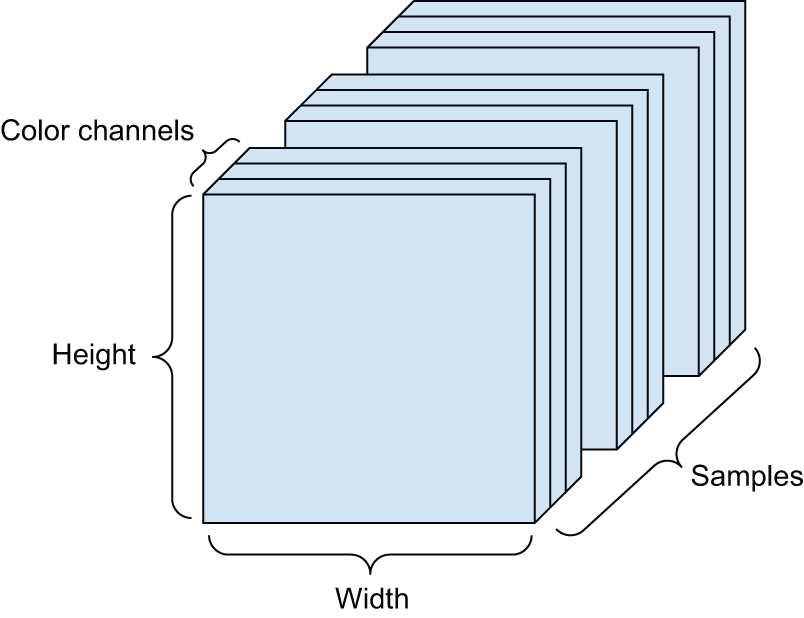
\includegraphics[width=\textwidth,height=0.7\textheight,keepaspectratio]{../../images/ch02/image_data.8accee38.png}
            \caption{Tensor 4D biểu diễn dữ liệu ảnh màu}
        \end{figure}
    \end{columns}
\end{frame}

\begin{frame}{Ví dụ thực tế: Dữ liệu Video}
    Dữ liệu video là trường hợp phức tạp nhất trong thực tế, sử dụng \textbf{Tensor 5D}.
    \begin{itemize}
        \item Một video là một chuỗi các khung hình (frames), mỗi frame là ảnh màu 3D.
        \item Hình dạng của tensor: \texttt{(mẫu, khung hình, chiều cao, chiều rộng, kênh màu)}
        \item \textit{Ví dụ:} Một lô 4 clip YouTube 60 giây ($144 \times 256$ pixels, 4 fps) có 240 khung hình sẽ có hình dạng \texttt{(4, 240, 144, 256, 3)}.
        \item Kích thước này rất lớn (tương đương $\sim 425$ MB cho kiểu \texttt{float32}).
    \end{itemize}
\end{frame}

% ---------------------------------------------
\section{3. Các phép toán Tensor và Hình học}
% ---------------------------------------------

\begin{frame}[fragile]{Phép toán Tensor: Element-wise và Broadcasting}
    \textbf{Phép toán theo phần tử (Element-wise):}
    \begin{itemize}
        \item Áp dụng độc lập cho từng mục trong tensor (Cộng, Trừ, Hàm ReLU...).
        \item Được thực thi song song qua BLAS siêu tốc trên kiến trúc GPU.
    \end{itemize}
    \textbf{Phát sóng (Broadcasting):}
    \begin{itemize}
        \item Cho phép tính toán giữa 2 tensor khác kích thước (VD: Ma trận + Vector).
        \item Tensor nhỏ được "lặp lại" dọc theo trục mới để khớp hình dạng.
    \end{itemize}
    \begin{lstlisting}[language=Python]
import numpy as np
X = np.random.random((32, 10))
y = np.random.random((10,))
Z = X + y # y tu dong phat song thanh (32, 10) roi moi cong.
    \end{lstlisting}
\end{frame}

\begin{frame}{Sản phẩm Tensor (Tích vô hướng - Dot Product)}
    \begin{columns}
        \column{0.5\textwidth}
        \begin{itemize}
            \item Không giống phép nhân từng phần tử, \textbf{Tích Tensor} (\texttt{matmul} hoặc toán tử \texttt{@}) là phép toán phổ biến nhất.
            \item \textbf{Tích ma trận:} Kết hợp các hàng ma trận 1 với cột ma trận 2.
            \item Khả năng tương thích hình dạng: \\ \texttt{(a, b) $\cdot$ (b, c) $\rightarrow$ (a, c)}
        \end{itemize}
        
        \column{0.5\textwidth}
        \begin{figure}
            \centering
            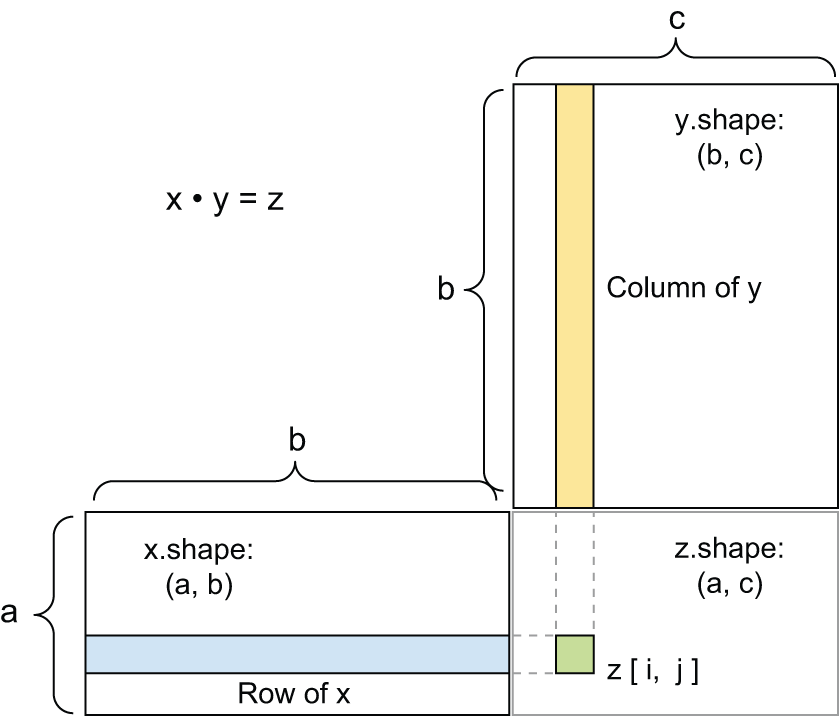
\includegraphics[width=\textwidth,height=0.7\textheight,keepaspectratio]{../../images/ch02/matrix_dot_box_diagram.3dc0f796.png}
            \caption{Sơ đồ hộp minh họa tích ma trận}
        \end{figure}
    \end{columns}
\end{frame}

\begin{frame}[fragile]{Định hình lại Tensor (Reshaping \& Transposing)}
    \begin{itemize}
        \item Định hình lại (Reshape) sắp xếp lại các hàng và cột để đạt được hình dạng mục tiêu mà không thay đổi tổng số phần tử.
    \end{itemize}
    \begin{lstlisting}[language=Python]
x = np.array([[0., 1.],
              [2., 3.],
              [4., 5.]]) # Shape: (3, 2)
x = x.reshape((6, 1)) # Tro thanh cot 6 phan tu
    \end{lstlisting}
    \begin{itemize}
        \item \textbf{Chuyển vị (Transpose):} Hoán đổi hàng thành cột.
    \end{itemize}
    \begin{lstlisting}[language=Python]
x = np.zeros((300, 20))
x = np.transpose(x) # Shape tro thanh (20, 300)
    \end{lstlisting}
\end{frame}

\begin{frame}{Ý nghĩa Hình học (1): Hàm số và Tính liên tục}
    \begin{columns}
        \column{0.5\textwidth}
        Tất cả phép toán tensor đều có ý nghĩa biến đổi hình học.
        \begin{itemize}
            \item Một mạng nơ-ron thực chất là một \textbf{hàm toán học} khổng lồ.
            \item Hàm số này phải \textbf{liên tục} và \textbf{trơn}.
        \end{itemize}
        
        \column{0.5\textwidth}
        \begin{figure}
            \centering
            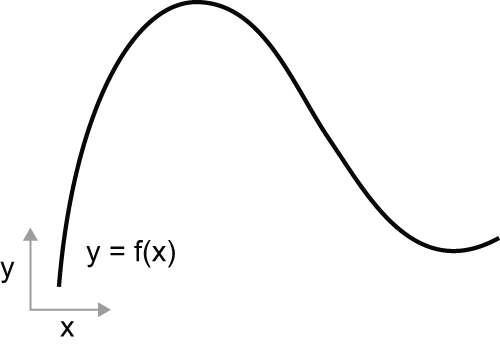
\includegraphics[width=0.8\textwidth,height=0.4\textheight,keepaspectratio]{../../images/ch02/function.4b000cb3.png}
            
            \vspace{0.2cm}
            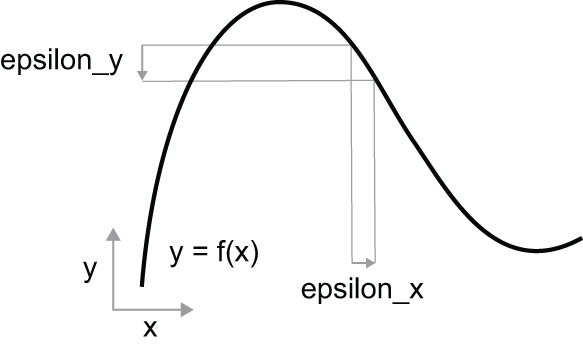
\includegraphics[width=0.8\textwidth,height=0.4\textheight,keepaspectratio]{../../images/ch02/continuity.98fd80b7.png}
            \caption{Sự liên tục: x thay đổi nhỏ dẫn đến y thay đổi nhỏ}
        \end{figure}
    \end{columns}
\end{frame}

\begin{frame}{Ý nghĩa Hình học (2): Tịnh tiến, Phóng to, Quay}
    \begin{columns}
        \column{0.33\textwidth}
        \begin{figure}
            \centering
            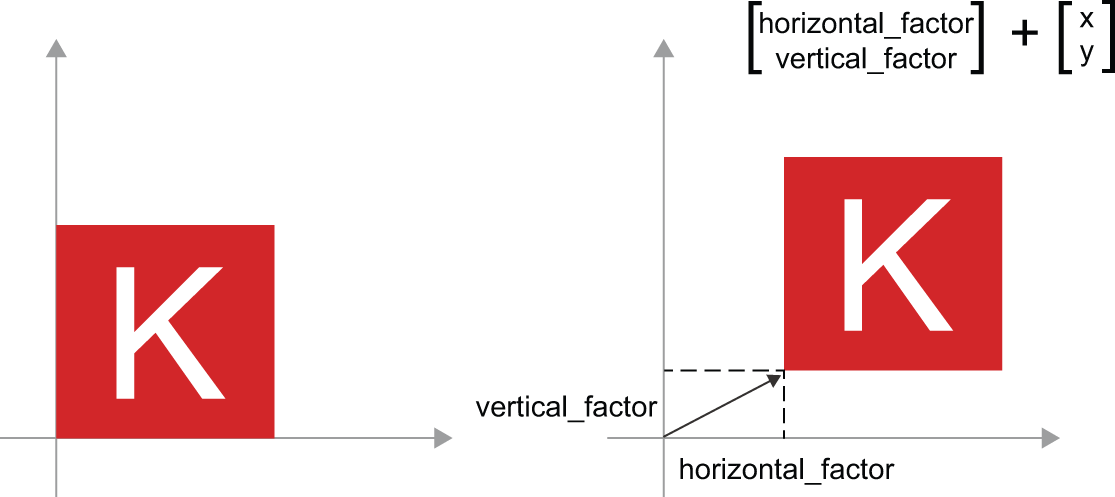
\includegraphics[width=\textwidth]{../../images/ch02/translation.c123da84.png}
            \caption{\textbf{Tịnh tiến:} Dời hình bằng phép cộng vector}
        \end{figure}
        
        \column{0.33\textwidth}
        \begin{figure}
            \centering
            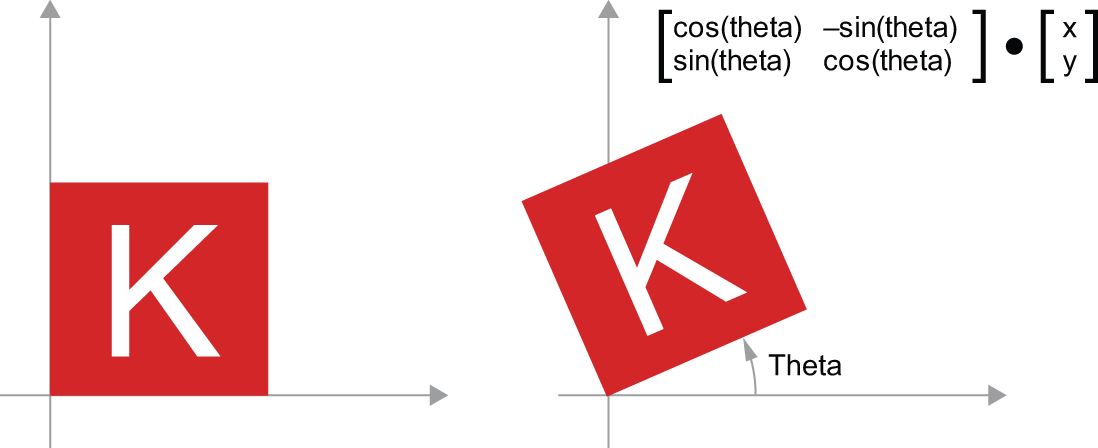
\includegraphics[width=\textwidth]{../../images/ch02/rotation.8f4da7c4.png}
            \caption{\textbf{Quay:} Tích ma trận $2 \times 2$ (Lượng giác)}
        \end{figure}
        
        \column{0.33\textwidth}
        \begin{figure}
            \centering
            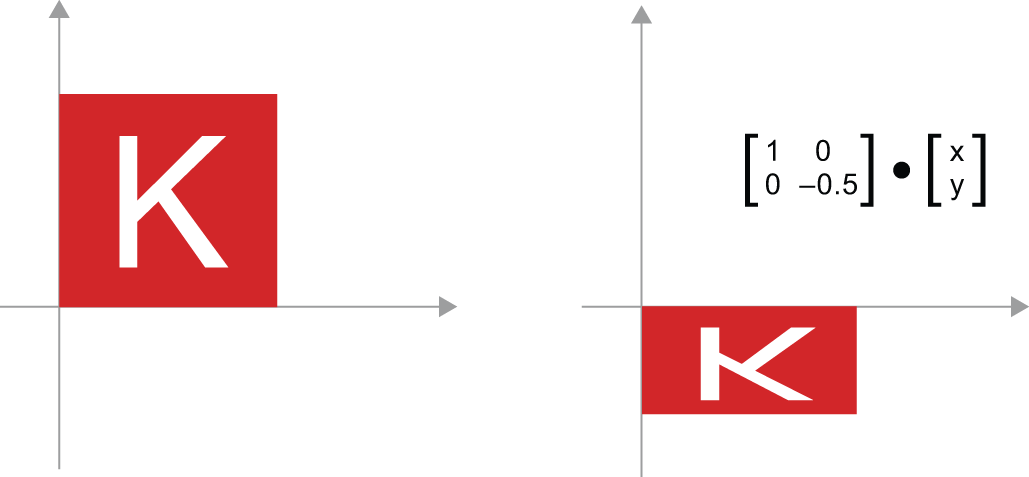
\includegraphics[width=\textwidth]{../../images/ch02/scaling.8cca5e17.png}
            \caption{\textbf{Thu phóng:} Tích ma trận đường chéo}
        \end{figure}
    \end{columns}
\end{frame}

\begin{frame}{Ý nghĩa Hình học (3): Phép biến đổi Affine \& Dense layer}
    \begin{columns}
        \column{0.5\textwidth}
        \begin{itemize}
            \item \textbf{Phép biến đổi Affine} là sự kết hợp của biến đổi tuyến tính (nhân $\mathbf{W}$) và tịnh tiến (cộng $\mathbf{b}$).
            \item Lớp \texttt{Dense}: $\mathbf{y} = \mathbf{W} \cdot \mathbf{x} + \mathbf{b}$.
            \item \textbf{Kích hoạt phi tuyến (ReLU):} Giúp bóp méo không gian affine, tạo ra các ranh giới phức tạp (để phân tách dữ liệu).
        \end{itemize}
        
        \column{0.5\textwidth}
        \begin{figure}
            \centering
            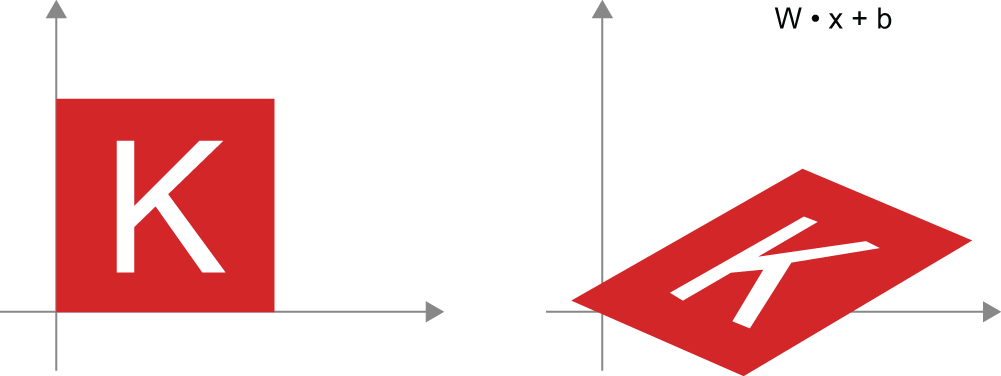
\includegraphics[width=0.8\textwidth]{../../images/ch02/affine_transform.80be4403.png}
            
            \vspace{0.2cm}
            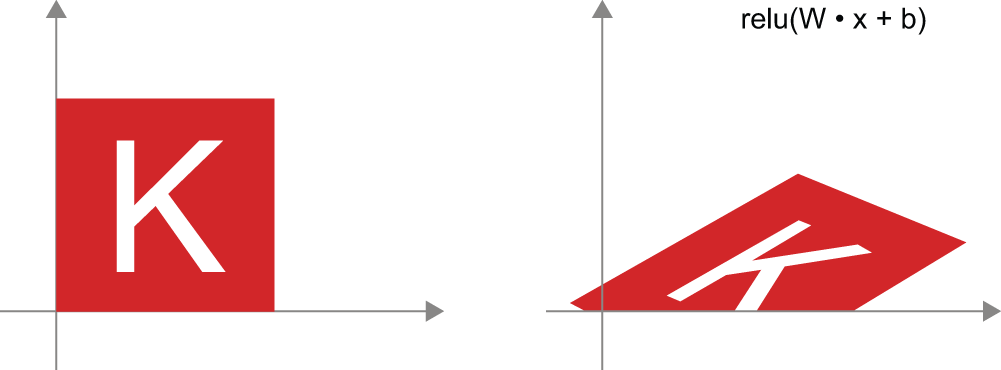
\includegraphics[width=0.8\textwidth]{../../images/ch02/dense_transform.d8a02328.png}
            \caption{Biến đổi Affine \& theo sau là ReLU}
        \end{figure}
    \end{columns}
\end{frame}

\begin{frame}{Ý nghĩa Hình học (4): Gỡ rối dữ liệu}
    Học sâu bản chất là chuỗi biến đổi hình học tinh vi để "gỡ rối" (untangle) các đa tạp dữ liệu phức tạp đan xen nhau.
    \begin{figure}
        \centering
        \begin{minipage}{0.24\textwidth}
            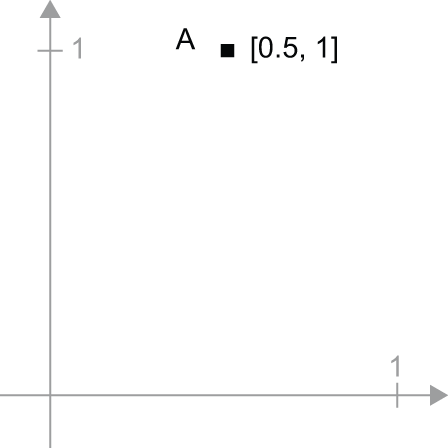
\includegraphics[width=\linewidth]{../../images/ch02/geometric_interpretation_1.4c2c1983.png}
        \end{minipage}
        \hfill
        \begin{minipage}{0.24\textwidth}
            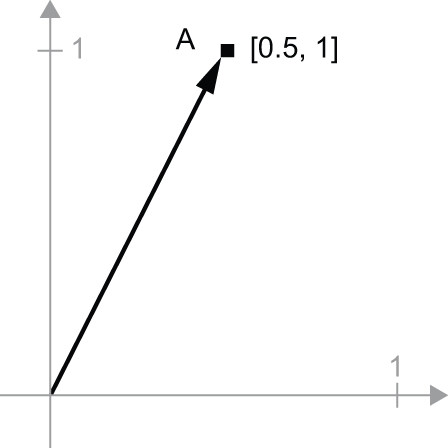
\includegraphics[width=\linewidth]{../../images/ch02/geometric_interpretation_2.e635ec60.png}
        \end{minipage}
        \hfill
        \begin{minipage}{0.24\textwidth}
            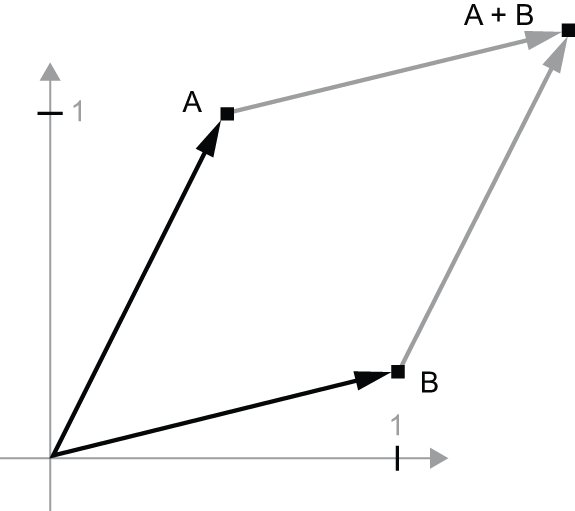
\includegraphics[width=\linewidth]{../../images/ch02/geometric_interpretation_3.b1b80fb9.png}
        \end{minipage}
        \hfill
        \begin{minipage}{0.24\textwidth}
            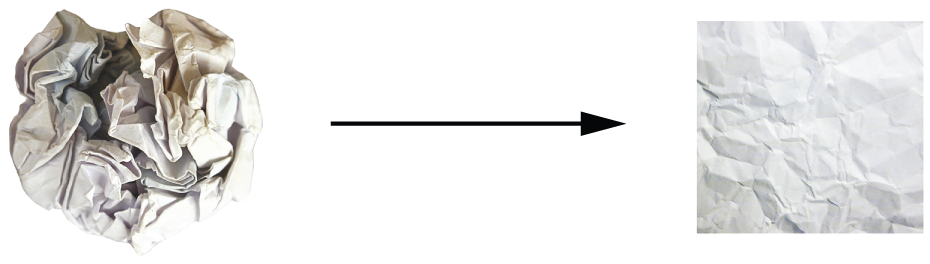
\includegraphics[width=\linewidth]{../../images/ch02/geometric_interpretation_4.f8123b83.png}
        \end{minipage}
        \caption{Quá trình phân tách dữ liệu qua các lớp ẩn giống như việc từ từ vuốt phẳng một quả bóng giấy vò nát.}
    \end{figure}
\end{frame}

% ---------------------------------------------
\section{4. Tối ưu hóa Dựa trên Gradient}
% ---------------------------------------------

\begin{frame}{Vòng lặp Đào tạo (Training Loop)}
    \begin{itemize}
        \item Khởi tạo ngẫu nhiên trọng số mô hình $\mathbf{W}$ và $\mathbf{b}$.
        \item Lặp lại các bước sau (Vòng lặp đào tạo):
        \begin{enumerate}
            \item Lấy một lô ngẫu nhiên dữ liệu huấn luyện $\mathbf{x}$ và nhãn $\mathbf{y\_true}$.
            \item \textbf{Forward Pass:} Chạy mô hình trên $\mathbf{x}$ để dự đoán $\mathbf{y\_pred}$.
            \item Tính hàm Mất mát (Loss) để đo lường sai số.
            \item Cập nhật tất cả các trọng số theo hướng giảm Loss.
        \end{enumerate}
        \item Làm sao để biết thay đổi trọng số bao nhiêu và hướng nào? Phương pháp: \textbf{Gradient Descent}.
    \end{itemize}
\end{frame}

\begin{frame}{Khái niệm Đạo hàm (Derivative)}
    \begin{columns}
        \column{0.5\textwidth}
        Đạo hàm $f'(x)$ thể hiện \textbf{độ dốc (slope)} của tiếp tuyến với hàm số $f(x)$ tại điểm $x$.
        \begin{itemize}
            \item Nếu $f'(x) > 0$, tăng $x$ sẽ làm hàm tăng.
            \item Nếu $f'(x) < 0$, tăng $x$ sẽ làm hàm giảm.
            \item $\Rightarrow$ Muốn giảm giá trị $f(x)$ (Loss), chỉ cần đi \textbf{ngược hướng} với đạo hàm.
        \end{itemize}
        
        \column{0.5\textwidth}
        \begin{figure}
            \centering
            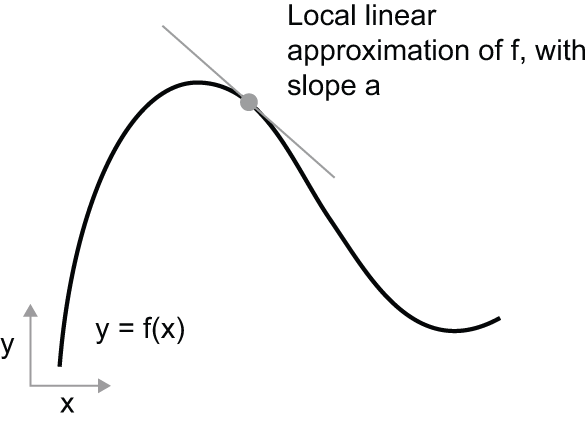
\includegraphics[width=\textwidth,height=0.7\textheight,keepaspectratio]{../../images/ch02/derivation.306de198.png}
            \caption{Đạo hàm là hệ số góc của tiếp tuyến}
        \end{figure}
    \end{columns}
\end{frame}

\begin{frame}{Đạo hàm của Tensor: Gradient}
    \begin{columns}
        \column{0.45\textwidth}
        Sự tổng quát hóa của đạo hàm trong không gian đa chiều (nhiều tham số trọng số) gọi là \textbf{Gradient}.
        \begin{itemize}
            \item Gradient biểu thị \textbf{độ cong} của bề mặt hàm Loss đa chiều.
            \item Vectơ Gradient luôn chỉ về hướng hàm $L$ tăng nhanh nhất.
            \item \textbf{Ngược hướng Gradient} là con đường ngắn nhất xuống thung lũng Loss.
        \end{itemize}
        
        \column{0.55\textwidth}
        \begin{figure}
            \centering
            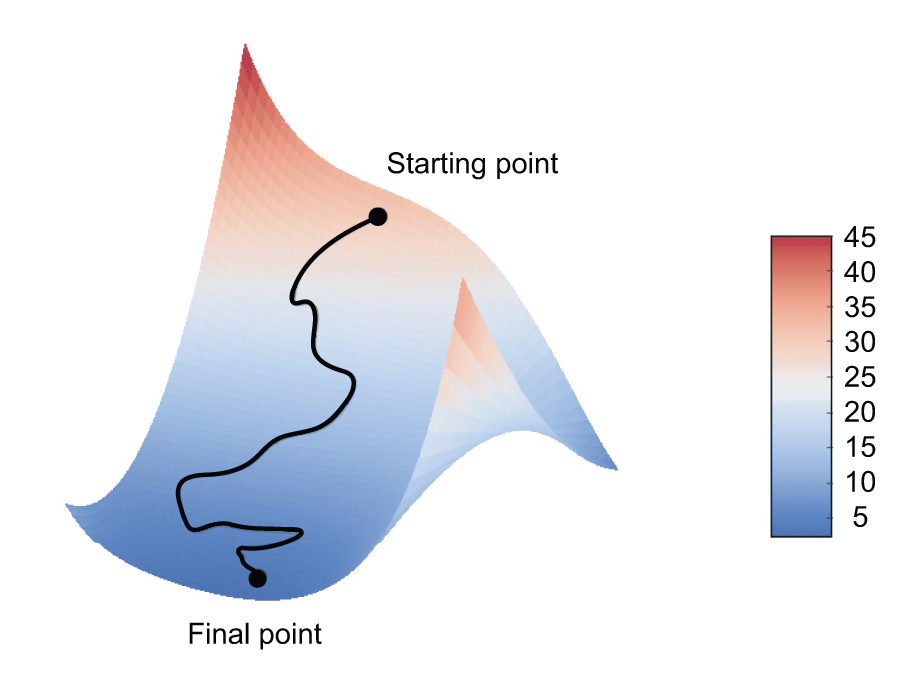
\includegraphics[width=\textwidth,height=0.7\textheight,keepaspectratio]{../../images/ch02/gradient_descent_3d.85d77c73.png}
            \caption{Mặt cong 3D của Loss function}
        \end{figure}
    \end{columns}
\end{frame}

\begin{frame}{Cực tiểu Toàn cục và Cực tiểu Cục bộ}
    \begin{columns}
        \column{0.5\textwidth}
        Mục tiêu của học sâu là tìm \textbf{Cực tiểu toàn cục (Global Minimum)}, nơi sai số đạt mức thấp nhất.
        \begin{itemize}
            \item Tại cực tiểu, Gradient bằng 0 ($\nabla L = 0$).
            \item Với bề mặt Loss phức tạp, mô hình rất dễ mắc kẹt tại \textbf{Cực tiểu cục bộ (Local Minimum)}.
        \end{itemize}
        
        \column{0.5\textwidth}
        \begin{figure}
            \centering
            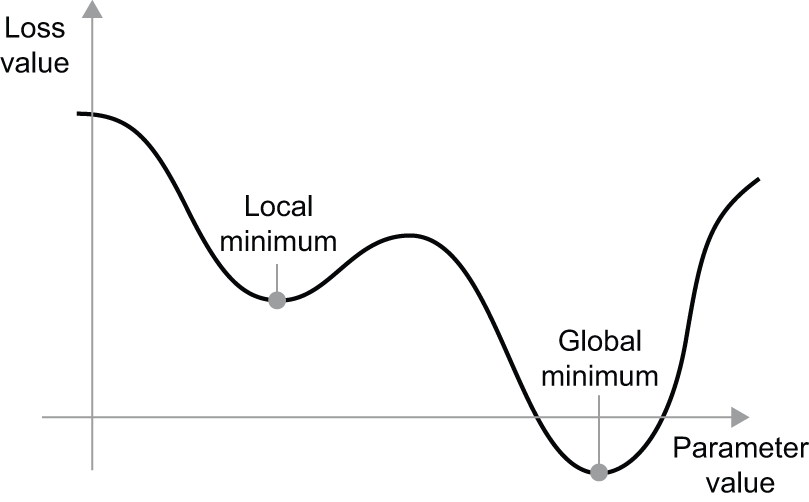
\includegraphics[width=\textwidth,height=0.7\textheight,keepaspectratio]{../../images/ch02/global_minimum.8f000c0a.png}
            \caption{Local Minimum vs Global Minimum}
        \end{figure}
    \end{columns}
\end{frame}

\begin{frame}{Thuật toán SGD và Momentum}
    \begin{columns}
        \column{0.5\textwidth}
        \textbf{Stochastic Gradient Descent (SGD):} Cập nhật dựa trên một mẻ nhỏ ngẫu nhiên.\\
        $W \leftarrow W - \text{learning\_rate} \times \nabla L$
        \begin{itemize}
            \item \textbf{Động lượng (Momentum):} Lấy cảm hứng từ một quả bóng lăn dốc, sử dụng vận tốc quá khứ để giúp quả bóng thoát khỏi các cực tiểu cục bộ hẹp.
        \end{itemize}
        
        \column{0.5\textwidth}
        \begin{figure}
            \centering
            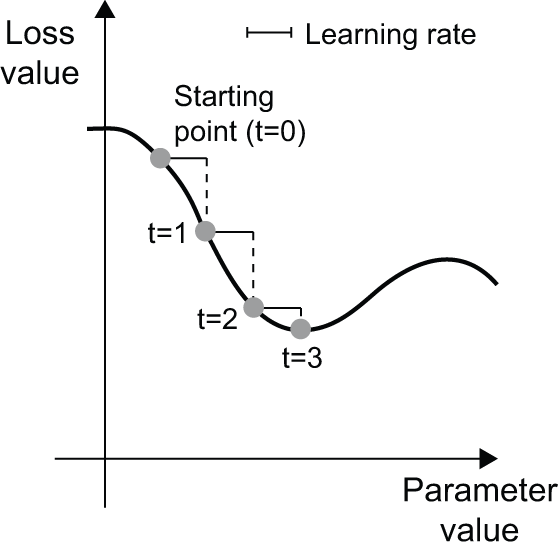
\includegraphics[width=\textwidth,height=0.4\textheight,keepaspectratio]{../../images/ch02/sgd_explained_1.0535e152.png}
            
            \vspace{0.2cm}
            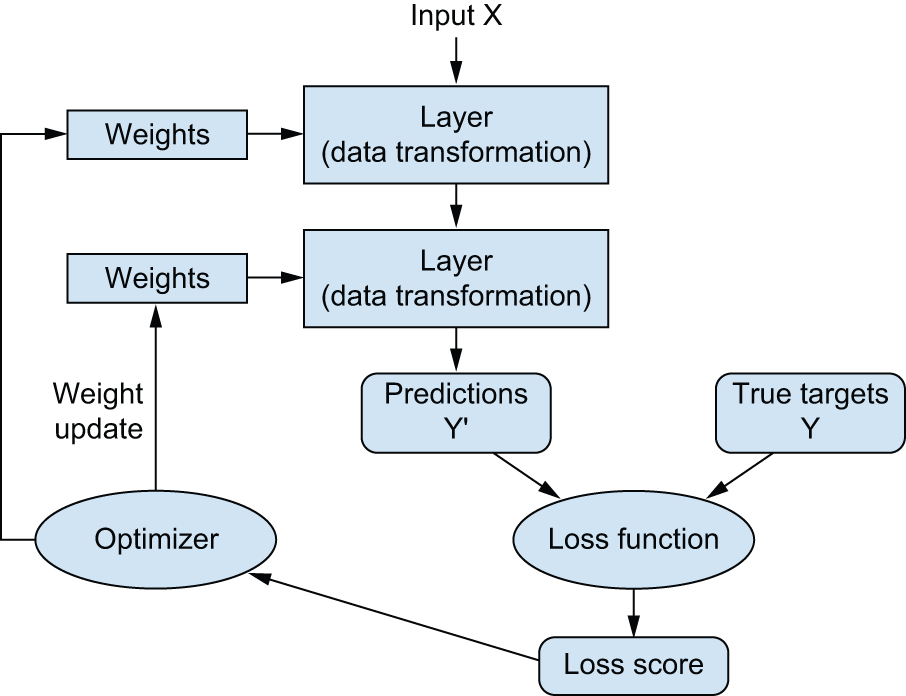
\includegraphics[width=\textwidth,height=0.35\textheight,keepaspectratio]{../../images/ch02/deep-learning-in-3-figures-3_alt.40aa865d.png}
            \caption{Hạ Gradient ngẫu nhiên \& Vòng lặp Optimizer}
        \end{figure}
    \end{columns}
\end{frame}

% ---------------------------------------------
\section{5. Đồ thị Tính toán \& Lan truyền ngược}
% ---------------------------------------------

\begin{frame}{Đồ thị Tính toán (Computation Graph)}
    \begin{columns}
        \column{0.5\textwidth}
        Làm sao để tính đạo hàm của hàng triệu trọng số? Sử dụng \textbf{Lan truyền ngược}.
        \begin{itemize}
            \item Cốt lõi của nó là \textbf{Đồ thị tính toán}. 
            \item Các phép toán Tensor trở thành các "nút" (node), dữ liệu trở thành các cạnh. 
            \item Biến tính toán toán học thành dữ liệu cấu trúc phục vụ máy tính.
        \end{itemize}
        
        \column{0.5\textwidth}
        \begin{figure}
            \centering
            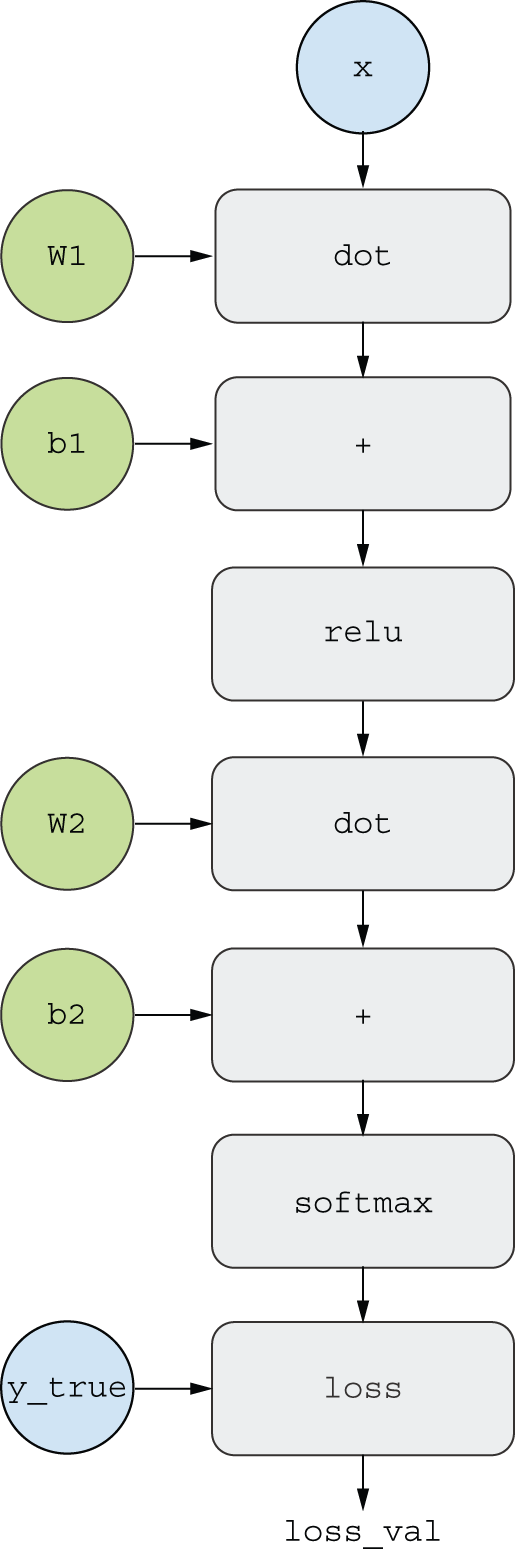
\includegraphics[width=\textwidth,height=0.7\textheight,keepaspectratio]{../../images/ch02/a_first_computation_graph.90dec1fc.png}
            \caption{Biểu diễn đồ thị cho mô hình mạng nơ-ron}
        \end{figure}
    \end{columns}
\end{frame}

\begin{frame}{Ví dụ lan truyền thuận (Forward Pass)}
    \begin{columns}
        \column{0.5\textwidth}
        Ví dụ cơ bản:\\
        $y = (x \cdot w) + b$\\
        Mất mát: $Loss = |y_{true} - y|$
        \begin{itemize}
            \item Tính toán đi từ input qua các phép toán đến output được gọi là \textbf{Lan truyền thuận}.
            \item Tại bước này, các giá trị Tensor được ghi nhớ trên các cạnh.
        \end{itemize}
        
        \column{0.5\textwidth}
        \begin{figure}
            \centering
            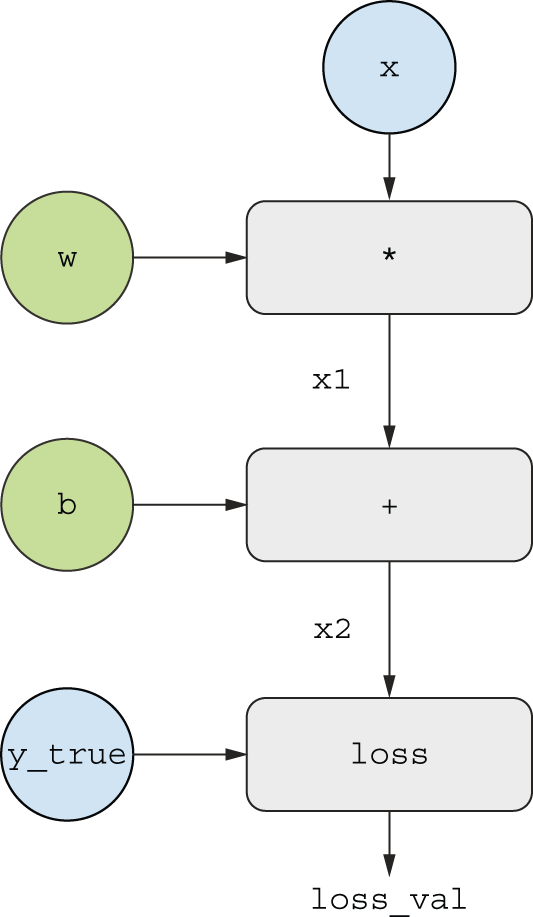
\includegraphics[width=0.8\textwidth]{../../images/ch02/basic_computation_graph.f3e3c75a.png}
            
            \vspace{0.1cm}
            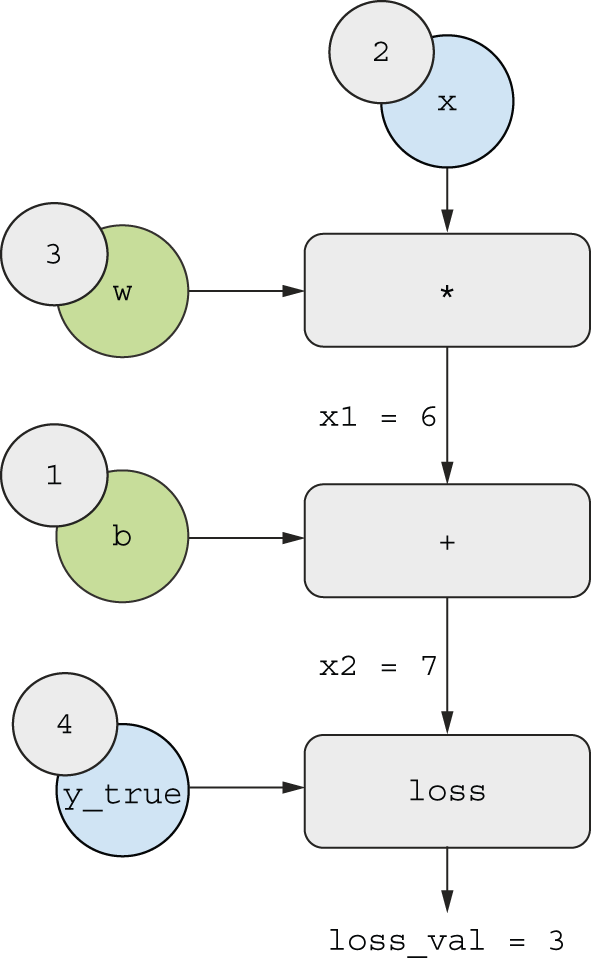
\includegraphics[width=0.8\textwidth]{../../images/ch02/basic_computation_graph_with_values.e15cd230.png}
            \caption{Tính giá trị theo chiều thuận}
        \end{figure}
    \end{columns}
\end{frame}

\begin{frame}{Lan truyền ngược (Backpropagation) \& Quy tắc Chuỗi}
    \begin{columns}
        \column{0.5\textwidth}
        Bằng cách áp dụng \textbf{Quy tắc chuỗi (Chain Rule)}:
        \[ \frac{d(f(g(x)))}{dx} = f'(g(x)) \cdot g'(x) \]
        \begin{itemize}
            \item Bắt đầu từ Loss, ta lan truyền đạo hàm \textbf{ngược về Input}.
            \item Đạo hàm toàn cục tới từng trọng số chính là tích của các đạo hàm cục bộ dọc theo đường đi (cạnh).
        \end{itemize}
        
        \column{0.5\textwidth}
        \begin{figure}
            \centering
            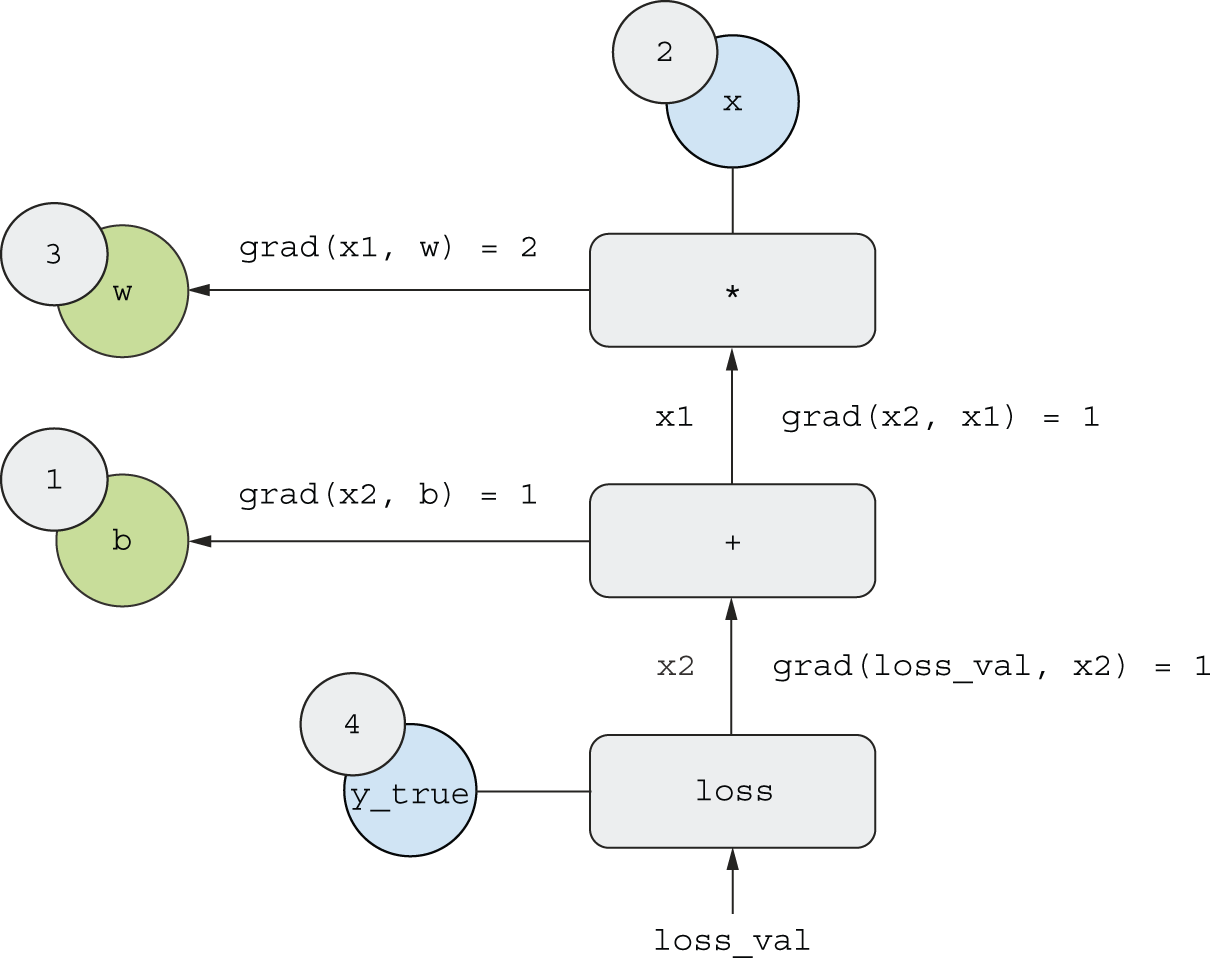
\includegraphics[width=\textwidth]{../../images/ch02/basic_computation_graph_backward.9e975200.png}
            
            \vspace{0.1cm}
            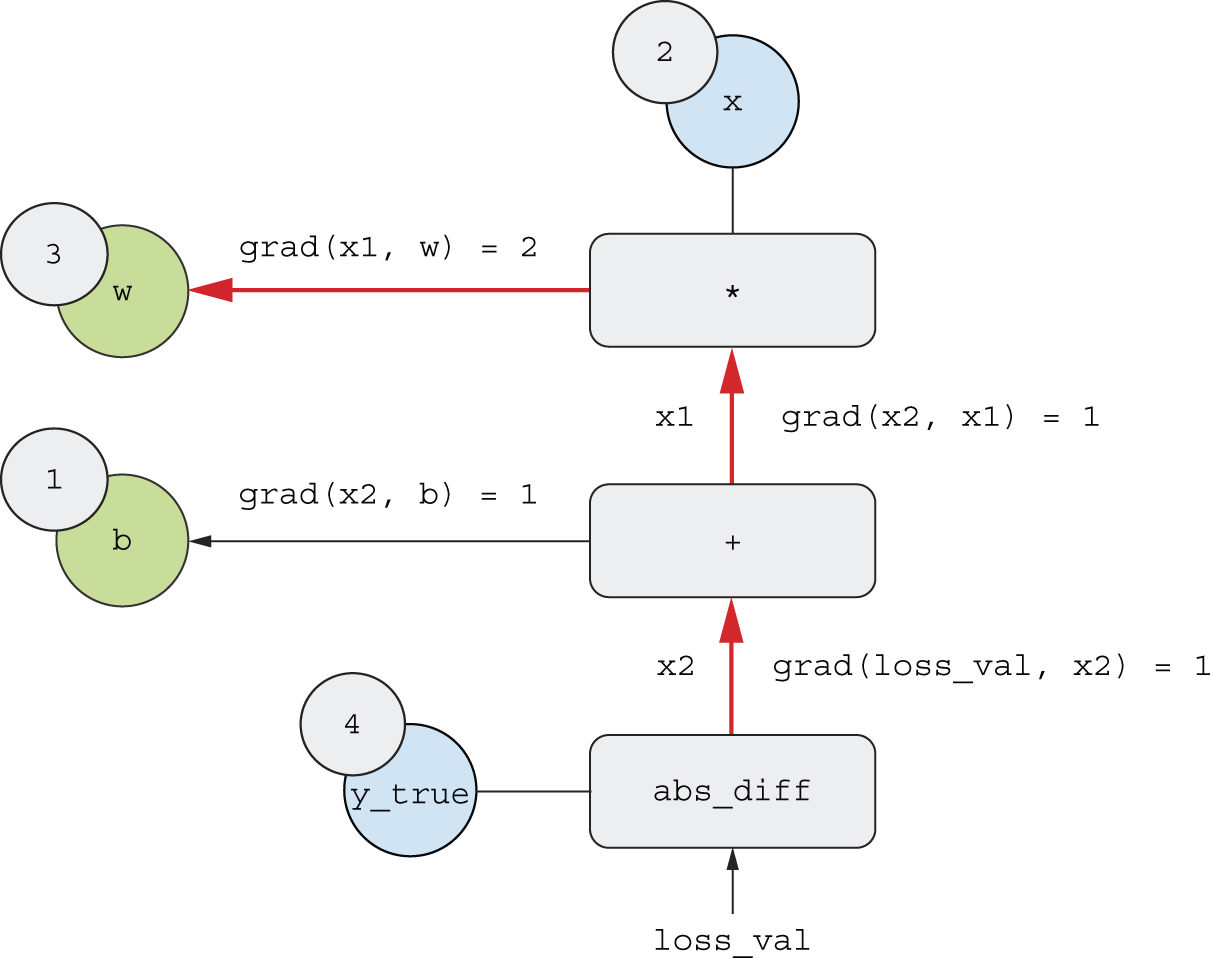
\includegraphics[width=\textwidth]{../../images/ch02/path_in_backward_graph.fe91e7d0.png}
            \caption{Nhân các đạo hàm cục bộ để thu đạo hàm Loss}
        \end{figure}
    \end{columns}
\end{frame}

\begin{frame}[fragile]{Tự động phân biệt với TensorFlow GradientTape}
    \begin{itemize}
        \item Thực tế, Framework hiện đại như TensorFlow tự động hóa toàn bộ việc Lan truyền ngược bằng \textbf{Automatic Differentiation}.
    \end{itemize}
    \begin{lstlisting}[language=Python]
import tensorflow as tf

x = tf.zeros(shape=()) # Gia tri khoi tao
with tf.GradientTape() as tape:
    # Tape (Bang ghi) se luu lai do thi cac phep toan 
    y = 2 * x + 3 

# Yeu cau Tape tinh gradient cua y doi voi x (dao ham)
grad_of_y_wrt_x = tape.gradient(y, x) 
    \end{lstlisting}
\end{frame}

\begin{frame}[fragile]{Thực hành (Từ đầu): NaiveDense}
    \begin{itemize}
        \item Hãy xây dựng thủ công một lớp \texttt{Dense} sử dụng tensor ops.
    \end{itemize}
    \begin{lstlisting}[language=Python]
import keras
from keras import ops

class NaiveDense:
    def __init__(self, input_size, output_size, activation=None):
        self.activation = activation
        self.W = keras.Variable(shape=(input_size, output_size), 
                                initializer="uniform")
        self.b = keras.Variable(shape=(output_size,), initializer="zeros")

    def __call__(self, inputs): # Thuc hien Forward Pass
        x = ops.matmul(inputs, self.W) + self.b
        if self.activation: 
            x = self.activation(x)
        return x
    \end{lstlisting}
\end{frame}

\begin{frame}[fragile]{Thực hành (Từ đầu): Vòng lặp Huấn luyện}
    \begin{itemize}
        \item Khái quát lại quá trình \texttt{model.fit()} bằng đoạn code sau:
    \end{itemize}
    \begin{lstlisting}[language=Python]
def one_training_step(model, images_batch, labels_batch):
    with tf.GradientTape() as tape:
        # 1. Forward pass de du doan va tinh Loss
        predictions = model(images_batch)
        loss = ops.sparse_categorical_crossentropy(labels_batch, predictions)
        average_loss = ops.mean(loss)
    
    # 2. Backward pass (Tinh gradient tu dong nho Tape)
    gradients = tape.gradient(average_loss, model.weights)
    
    # 3. Cap nhat trong so bang Optimizer (nhu SGD)
    update_weights(gradients, model.weights)
    
    return average_loss
    \end{lstlisting}
\end{frame}

\begin{frame}{Tổng kết Chương 2}
    \begin{itemize}
        \item \textbf{Tensors:} Nền tảng cấu trúc dữ liệu của học sâu. Bao gồm các bậc 0D, 1D, 2D, 3D, 4D v.v.
        \item \textbf{Phép toán Tensor:} Phép nhân ma trận, phép cộng, ReLU... là những biến đổi hình học tinh vi giúp gỡ rối đa diện dữ liệu.
        \item \textbf{Trọng số (Weights):} Tham số học hỏi chứa toàn bộ "kiến thức" của mô hình mạng.
        \item \textbf{Loss function \& Optimizers:} Loss đo lường độ chính xác (mục tiêu cần tối thiểu hóa). Optimizer như SGD giảm Loss thông qua đi ngược Gradient.
        \item \textbf{Backpropagation:} Sử dụng Đồ thị tính toán và Quy tắc chuỗi để tính đạo hàm ngược một cách nhanh chóng qua cơ chế phân biệt tự động (\texttt{GradientTape}).
    \end{itemize}
\end{frame}

\end{document}
